\chapter{Vật lý hiện đại}
\section{Thuyết tương đối và hệ quả}
\subsection{Phép biến đổi Galileo và Lorentz}
Phép biến đổi Galileo được xây dựng từ chuyển động trong hệ quy chiếu quán tính (tức là hệ quy chiếu không có gia tốc). 
Xét hệ quy chiếu K đứng yên, có hệ tọa độ Oxyz gắn với nó và một hệ quy chiếu K' chuyển động đều với vận tốc v dọc theo trục Ox. Ta thiết lập phép biến đổi Galileo từ hệ quy chiếu K sang K'
\begin{figure}
    \centering
    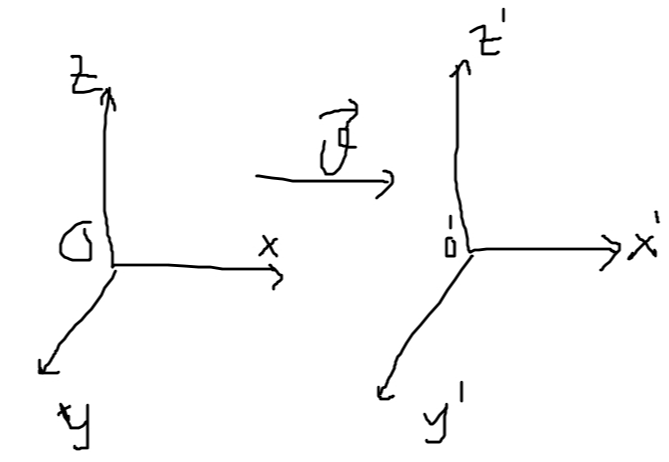
\includegraphics[width=0.5\textwidth]{galileo.png}
    \caption{Phép biến đổi Galileo}
    \label{galileo}
\end{figure}
$$\left\{\begin{array}{ll}
    x'=x-vt     &  \\
    y'=y     &\\
    z'=z & \\
    t'=t & \\
    \end{array}\right.$$
Dễ nhận thấy rằng trong phạm vi của cơ học cổ điển thì thời gian có tính tuyệt đối, không gian có tính tương đối và khối lượng của vật là bất biến. Thế nhưng, khi 
vật di chuyển với gần vận tốc ánh sáng, khối lượng của vật không còn bất biến nữa thì phép biến đổi Galileo không còn chính xác. Khi đó ta có phép biến đổi Lorentz như sau:
$$\left\{\begin{array}{ll}
    x'=\frac{x-vt}{\sqrt{1-\frac{v^2}{c^2}}}    &  \\
    y'=y     &\\
    z'=z & \\
    t'=\frac{t-\frac{v}{c^2}x}{\sqrt{1-\frac{v^2}{c^2}}} & \\
    \end{array}\right.$$
Đây là phép biến đổi Lorentz từ hệ quy chiếu K sang K'.
\subsection{Hệ quả của thuyết tương đối}
Ngoài ra, khi vật chuyển động với gần vận tốc ánh sáng, ta cũng cần lưu ý thêm một số công thức sau:
$$m=\frac{m_{0}}{\sqrt{1-\frac{v^2}{c^2}}}$$
$$l'=l\sqrt{1-\frac{v^2}{c^2}}$$
$$t'=t\sqrt{1-\frac{v^2}{c^2}}$$
$$E=mc^2=\frac{E_{0}}{\sqrt{1-\frac{v^2}{c^2}}}$$
$$E=hf=\frac{hc}{\lambda}$$ 
\section{Lưỡng tính sóng hạt}
Một photon có vận tốc gần với tốc độ ánh sáng sẽ vừa có tính sóng và vừa có tính hạt, ta có biến đổi sau:
$$E=hf=\frac{hc}{\lambda}=pc\Rightarrow \lambda=\frac{h}{p}$$
De Broglie cho rằng phương trình trên cũng có thể áp dụng được với các loại hạt khác ngoài photon, và bước sóng De Broglie của một hạt bất kì là:
$$\lambda=\frac{h}{mv}$$
Đây là phần câu hỏi đã được hỏi rất nhiều trong các đề thi gần đây nên hãy đọc thêm các tài liệu khác nữa để học.
\section{Vận tốc vũ trụ}
\begin{enumerate}
    \item Vận tốc vũ trụ cấp 1: Là vận tốc tối thiểu truyền vào cho vật để nó trở thành vệ tinh của trái đất.
    $$G\frac{Mm}{R^2}=\frac{mv_{1}^2}{R}\Rightarrow v_{1}=\sqrt{\frac{GM}{R}}$$
    \item  Vận tốc vũ trụ cấp 2: Là vận tốc tối thiểu truyền vào cho vật để nó trở thành hành tinh trong hệ mặt trời.
    $$G\frac{Mm}{R}=\frac{mv_{2}^2}{2}\Rightarrow v_{2}=\sqrt{\frac{2GM}{R}}$$
    \item  Vận tốc vũ trụ cấp 3: Là vận tốc tối thiểu truyền vào cho vật để nó rời khỏi hệ mặt trời
    $$v_{3}=\sqrt{30Rg}-29.5$$
\end{enumerate}
Phần này cũng ra rất nhiều nên hãy học kĩ.
